\chapter{Introduction}

Este é o capítulo introdutório com exemplo de uma referência padrão. \textbf{Ressalta-se que o texto: ``Citado na página
...'' é opcional e que outras formatações também podem ser usadas.}
 

\chapter{Comandos básicos do \LaTeX \label{cap1}}


Aqui apresentamos os comandos mais básicos para preparação de um trabalho em \LaTeX. Para mais detalhes sugere-se, por exemplo, ``The
not so short introduction to  \LaTeX\  2$\varepsilon$'', que pode ser obtido em
\url{http://tug.ctan.org/info/lshort/english/lshort.pdf} e o manual da classe \abnTeX\ que foi a classe utilizada
na confecção deste modelo. Perceba que há links no arquivo pdf que permitem clicar sobre o número da referência e ser enviado para
lista de referências e que na última podem ser colocados links para os documentos referenciados.

Comentários em um arquivo \LaTeX\  podem ser introduzidos através do caracter \%. 

\section{Dicas gerais}

A principal dica que daremos neste texto é quanto ao \emph{Character Encoding} a ser usado nos arquivos. A classe \abnTeX, utilizada na
confecção deste modelo, é baseada no \emph{encoding} UTF-8. Desta forma, recomenda-se fortemente que \textbf{todos} os arquivos sigam
este padrão para não haver problemas com acentos, por exemplo. Isto pode ser facilmente configurado na grande maioria dos editores
\LaTeX.

Outra dica importante ao usar o  \LaTeX\ na confecção de trabalhos longos é que se pode dividir o arquivo fonte em vários arquivos e
usar os comandos \verb+\input{arquivo}+ e \verb+\include{arquivo}+. Esta estrutura foi adotada na confecção deste modelo. As diferenças
entre os dois comandos é que no primeiro não são criados os arquivos auxiliares para o arquivo incluído e seu conteúdo não
necessariamente se iniciam em uma nova página, enquanto no segundo arquivos auxiliares próprios são criados e o seu conteúdo se inicia
em uma nova página. A recomendação é que pequenos trechos do trabalho sejam incluídos com o comando \verb+\input+ enquanto trechos
maiores, como um capítulo, por exemplo, sejam incluídos através do comando \verb+\include+. Ao utilizar vários arquivos, apenas o
arquivo fonte principal deve ser compilado. Recomenda-se o uso de editores   \LaTeX\ que permitam a criação de projetos, o que facilita
ainda mais a navegação pelos vários arquivos, a compilação, visualização, etc.  Alguns editores recomendados são: TeXmaker (Linux, Mac,
Windows), TeXstudio (Linux, Mac, Windows), TeXnicCenter (Windows), Kile (Linux). 

\section{Incluindo referências}

Uma das grandes vantagens no uso do \LaTeX\ na confecção de trabalhos acadêmicos é a facilidade de se incluir, numerar e gerenciar
referências bibliográficas através de pacotes como o BibTeX. Desta forma, recomendamos o uso do último para gerenciar suas referências.
A grande maioria dos editores de revistas científicas, assim como o google books e outros sites fornecem arquivos com os dados
bibliográficos em formato BibTeX. Assim, basta criar um arquivo, com extensão \verb+.bib+, que contenha os dados das referências usadas
e adicioná-lo ao arquivo fonte, em local apropriado, através do comando \verb+\bibliography{nome_do_arquivo.bib}+. É importante
salientar que o uso correto do BibTeX depende de uma compilação inicial do arquivo fonte \LaTeX, seguida da compilação BibTeX e mais
duas compilações   \LaTeX. Isto permite a criação da lista de referências e o correto ordenamento destas ao longo do texto e na seção
de referências. De fato, o arquivo \verb+.bib+ pode conter muito mais referências que as efetivamente utilizadas no texto de forma que
apenas as que forem citadas no texto serão incluídas na seção de referências.  Além disso, a formatação que será dada à lista de
referências, assim como as informações disponíveis no arquivo \verb+.bib+ que serão efetivamente utilizadas, são definidas pelo padrão
adotado para as referências. Sugere-se que o formato a ser adotado seja o formato \verb+unsrt+ que foi selecionado neste documento
através dos comandos:\\ \verb+\usepackage[fixlanguage]{babelbib}+\\ \verb+\selectbiblanguage{brazil}+\\
\verb+\bibliographystyle{babunsrt}+\\ em locais apropriados. Além disso, alguns dos editores recomendados anteriormente permitem o
gerenciamento inclusive das referências ao se criar um projeto, o que facilita enormemente a inclusão de novas citações no texto.

Cada entrada do arquivo \verb+.bib+ tem estrutura similar à mostrada abaixo:
\begin{verbatim}
    @article{exemplo,
    author={ R. M. Herman and A. Asgharian},
    journal={J. Mol. Spectrosc.},
    volume={19},
    pages={305},
    year={1966},
    }
\end{verbatim}

Para fazer uma citação à esta referência basta incluir o comando \verb+\cite{exemplo}+, o que produz:. A formatação dada
a cada entrada depende do estilo selecionado. Para exemplificar, seguem citações a vários documentos que foram retiradas dos modelos do
\abnTeX\:.
\textbf{Ressalta-se que o texto: ``Citado na página ...'' presente na lista de referências é opcional e que outras formatações podem
ser usadas.}

\newpage


\section{\label{estruturacao}Estruturação do texto}

Para iniciar este capítulo utilizamos o comando \\ \verb+\chapter{Comandos básicos do \LaTeX \label{cap1}}+.\\ O comando
\verb+\label{cap1}+ é opcional e foi introduzido para permitir posteriores referências ao capítulo. Por exemplo, o comando
\verb+\ref{cap1}+, produz o seguinte resultado: \ref{cap1}, e pode ser usado para fazer referências a este capítulo ao longo do texto.
A numeração é automaticamente atualizada caso um novo capítulo seja introduzido. De fato, qualquer parte do texto, figuras, tabelas,
equações, etc podem ser nomeadas pelo comando \verb+\label+ e posteriormente referenciadas pelo comando \verb+\ref+.

Seções dentro de um capítulo podem ser introduzidas pelo comando \\ \verb+\section{\label{estruturacao}Estruturação do texto}+. \\
Subseções são incluídas com o comando \verb+\subsection{Nome da subseção}+. Pode-se também usar \verb+\subsubsection+ e assim por
diante. Caso o capítulo ou seção tenham um nome muito grande pode-se optar por introduzir um  nome resumido para o sumário e cabeçalho
das páginas usando, por exemplo, \verb+\section[título resumido]{título longo}+.

\section{Equações, figuras e tabelas}

\subsection{Equações}

Equações podem ser inseridas através do ambiente \verb+equation+. Como exemplo, o comando:
\begin{verbatim}
\begin{equation}
\label{Z1}
Z=\sum_E g(E) e^{-\beta E}=e^{-\beta \epsilon_0}\sum_n g_n \left 
( e^{-\beta \epsilon}\right )^n=e^{-\beta \epsilon_0}\sum_n g_n z^n,
\end{equation}
\end{verbatim}
produz a seguinte equação:
\begin{equation}
\label{Z1}
Z=\sum_E g(E) e^{-\beta E}=e^{-\beta \epsilon_0}\sum_n g_n \left 
( e^{-\beta \epsilon}\right )^n=e^{-\beta \epsilon_0}\sum_n g_n z^n,
\end{equation}
Podemos, então, no texto introduzir facilmente referências à equação \ref{Z1} usando o comando \verb+\ref{Z1}+.

\subsection{Figuras}

Figuras podem ser introduzidas usando o comando, retirado da Ref.~:
\begin{verbatim}
\begin{figure}[htb]
	\caption{\label{fig_grafico}Gráfico produzido em Excel e salvo como PDF}
	\begin{center}
	    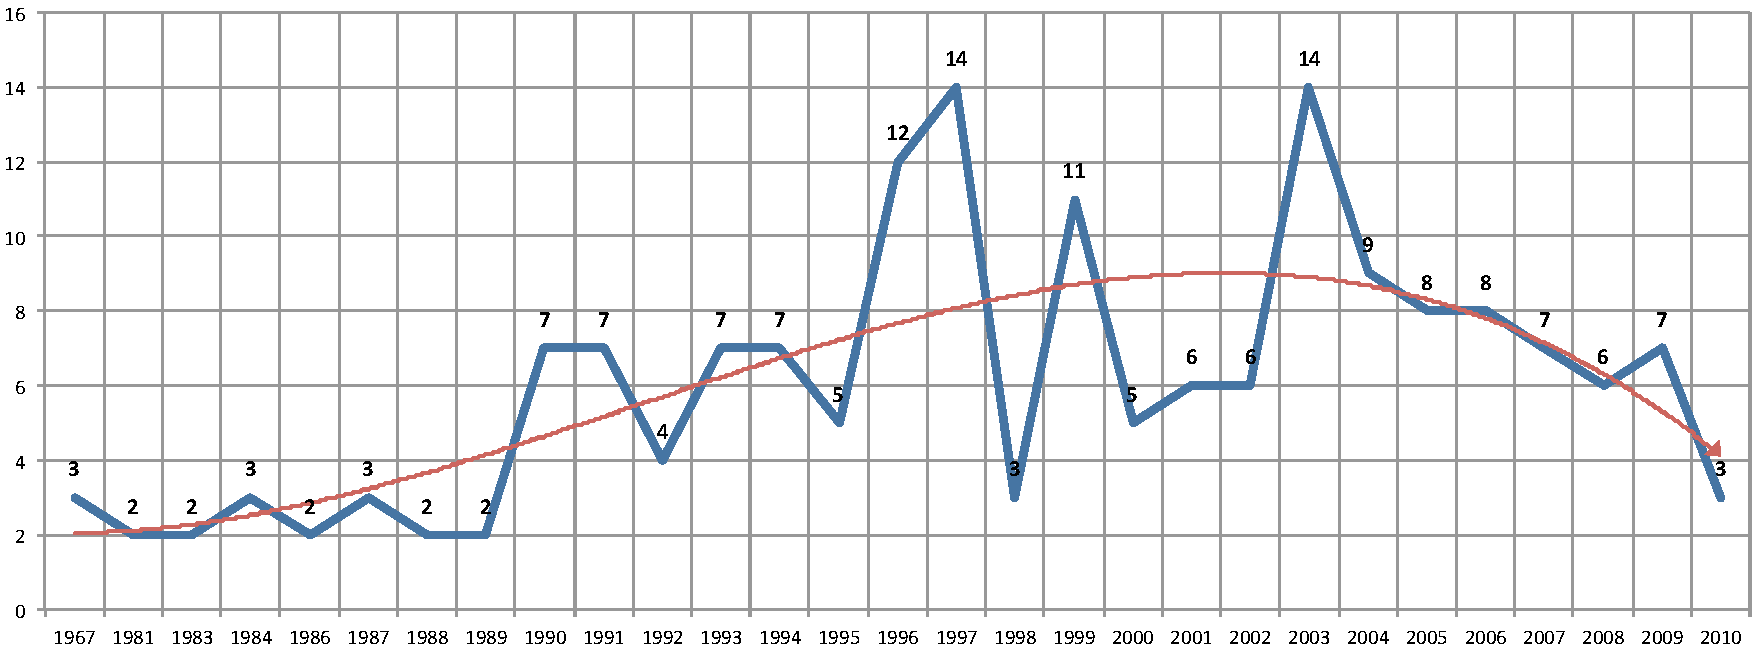
\includegraphics[scale=0.5]{fig/abntex2-modelo-img-grafico.pdf}
	\end{center}
	\legend{Fonte: \cite[p. 24]{araujo2012}}
\end{figure}
\end{verbatim}

Ressalta-se que ao invés de estabelecer a escala da figura através do comando \verb+scale=0.5+, poderia-se definir sua largura ou
altura através de \verb+width+ ou \verb+height+ usando, por exemplo, \\
\verb+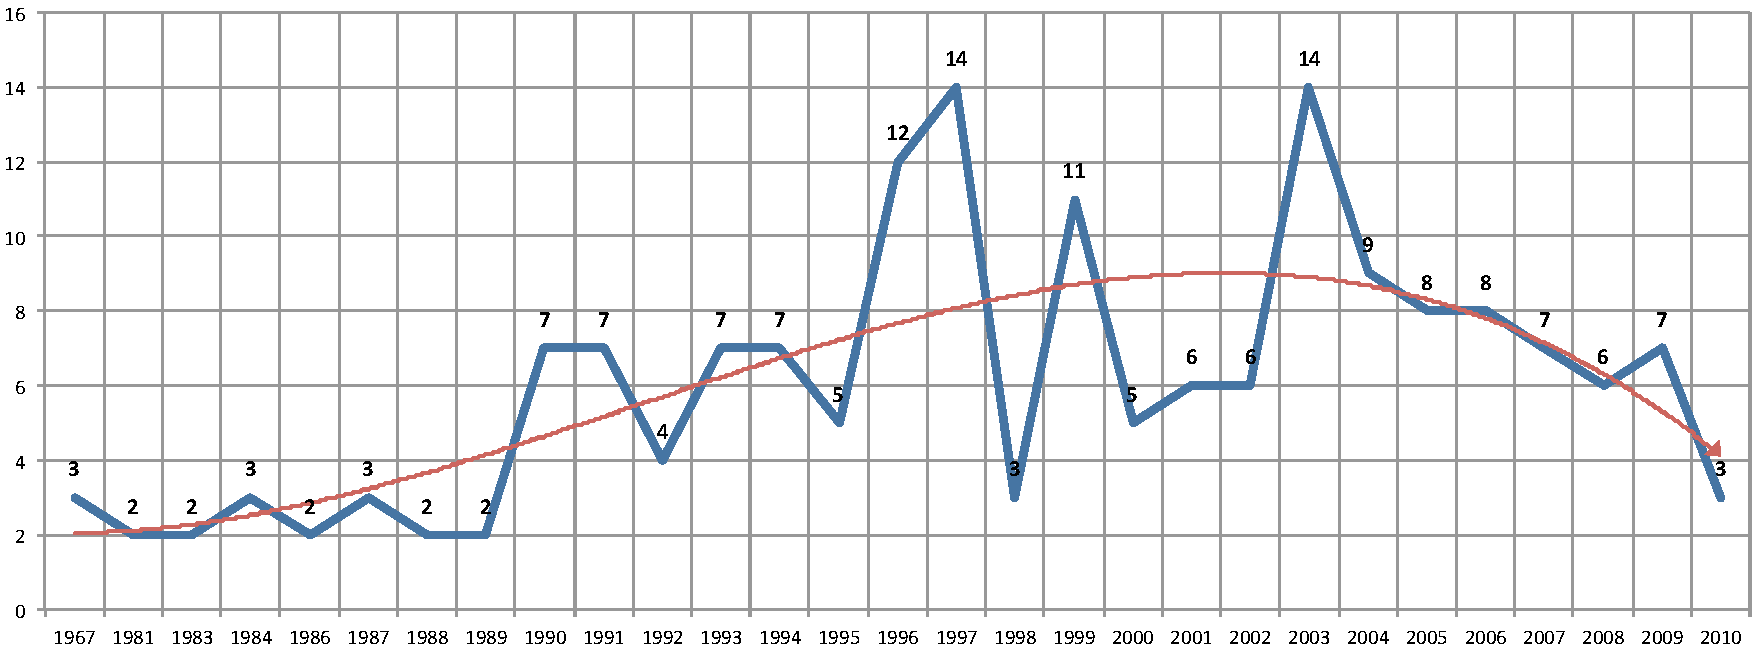
\includegraphics[width=5cm]{fig/abntex2-modelo-img-grafico.pdf}+ que re-escalaria a figura de forma a ela ficar com 5 cm de
largura. Pode-se ainda usar \verb+0.5\linewidth+ ao invés de \verb+5cm+ para estabelecer a largura da figura como sendo metade da
largura da linha do texto. O posicionamento da figura é definido pelo próprio \LaTeX. Recomenda-se colocar o comando o mais próximo
possível do lugar onde a figura é citada. Por fim, recomenda-se usar figuras em formato \verb+pdf+.

\begin{figure}[htb]
	\caption{\label{fig_grafico}Gráfico produzido em Excel e salvo como PDF}
	\begin{center}
	    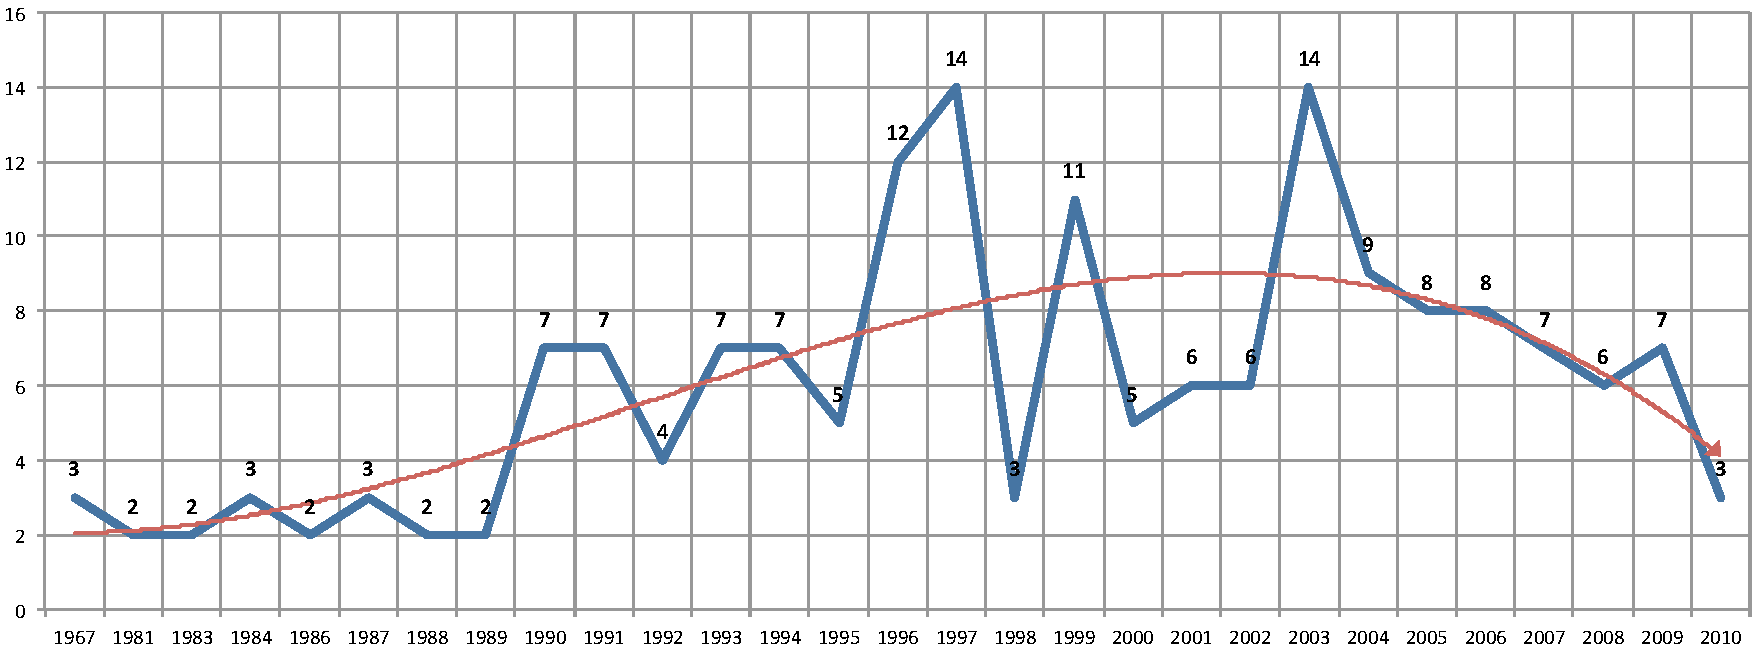
\includegraphics[scale=0.5]{fig/abntex2-modelo-img-grafico.pdf}
	\end{center}
	\legend{Fonte:}
\end{figure}


\subsection{Tabelas}

Há de se admitir que a confecção de tabelas em \LaTeX\ envolve uma prática um pouco maior. Abaixo apresentamos o comando que gerou a
Tabela~\ref{tab1}. Uma dica interessante é que o comando \verb+\resizebox+ permite ajustar a tabela à largura do texto e é
especialmente útil em situações onde a largura da tabela seria maior que a largura do texto.
\begin{scriptsize}
\begin{verbatim}
\begin{table}[ht] 
    \caption{Publicações relacionadas a alguma área em periódicos selecionados.
    \label{tab1}}
		\resizebox{\linewidth}{!}{%
\begin{tabular}{|l|c|c|c|c|c|c|c|c|c|}
    \hline
\multirow{2}{*}{\textbf{PERIÓDICO}} & \multicolumn{9}{c|}{ANOS}
\\ \cline{2-10}
& 2009&	2010&	2011&	2012&	2013&	2014&	2015& 2016& 2017\\ \hline
\textit{International Journal of Something} &	13&	15&	16&	15&	17&	17&	22& 22& 14\\ \hline 
\textit{Text Horizons}               		& 	6&	6&	9&	6&	8&	7&	19& 7& 6\\ \hline 
\textit{The Blablabla Review}             & 	8&	14&	9&	9&	15&	13&	21& 15& 9\\ \hline 
\textit{Journal of Magic}		&	2&	4&	2&	5&	1&	5&	1& 7& 4\\ \hline 
\textbf{TOTAL}&                           	29&	39&	36&	35&	41&	42&	63& 51& 33\\ \hline 
\multicolumn{8}{l}{Confeccionado pelo autor.}
\end{tabular}%
}
\end{table}
\end{verbatim}
\end{scriptsize}

\begin{table}[ht] 
    \caption{Publicações relacionadas a alguma área em periódicos selecionados.
    \label{tab1}}
		\resizebox{\linewidth}{!}{%
\begin{tabular}{|l|c|c|c|c|c|c|c|c|c|}
    \hline
\multirow{2}{*}{\textbf{PERIÓDICO}} & \multicolumn{9}{c|}{ANOS}
\\ \cline{2-10}
& 2009&	2010&	2011&	2012&	2013&	2014&	2015& 2016& 2017\\ \hline
\textit{International Journal of Something} &	13&	15&	16&	15&	17&	17&	22& 22& 14\\ \hline 
\textit{Text Horizons}               		& 	6&	6&	9&	6&	8&	7&	19& 7& 6\\ \hline 
\textit{The Blablabla Review}             & 	8&	14&	9&	9&	15&	13&	21& 15& 9\\ \hline 
\textit{Journal of Magic}		&	2&	4&	2&	5&	1&	5&	1& 7& 4\\ \hline 
\textbf{TOTAL}&                           	29&	39&	36&	35&	41&	42&	63& 51& 33\\ \hline 
\multicolumn{8}{l}{Confeccionado pelo autor.}
\end{tabular}%
}
\end{table}


\chapter{Conclusions}

Conclusões.

